\documentclass{../../res/univ-projet}

%Import des packages utilisés pour le document

% minted : http://www.ctan.org/tex-archive/macros/latex/contrib/minted/
% pour installer sur ubuntu:
% http://tex.stackexchange.com/questions/40083/how-to-install-minted-in-ubuntu#40101

\usepackage{lscape}
\usepackage{listings}
\usepackage{minted}
\usepackage{multicol}
\usepackage{color}

\usepackage{tikz}
\usetikzlibrary{arrows,positioning,shapes}
\tikzset{
  linea/.style ={draw,-stealth', rounded corners=1pt, line width=2pt},
  lineb/.style ={draw,-stealth', rounded corners=1pt, line width=2pt,color=blue!40!white},
  cell/.style = {rectangle, draw, fill=gray!60!white, text width=2cm,outer sep=0pt},
  cellx/.style = {rectangle,draw, fill=red!30!white, text width=1.5cm,outer sep=0pt}
}

\definecolor{success}{HTML}{198C19}
\definecolor{danger}{HTML}{CC0000}
\definecolor{bg-gray}{HTML}{F9F9F9}

%\usepackage{array}
%\usepackage{hyperref}
%\usepackage{tabularx, longtable}
%\usepackage[table]{xcolor}
%\usepackage{fancyhdr}
%\usepackage{lastpage}


\definecolor{gris}{rgb}{0.95, 0.95, 0.95}

%Redéfinition des marges
%\addtolength{\hoffset}{-2cm}
%\addtolength{\textwidth}{4cm}
\addtolength{\topmargin}{-1cm}
\addtolength{\textheight}{1cm}
\addtolength{\headsep}{0.8cm} 
\addtolength{\footskip}{-0.2cm}


%Import page de garde et structures pour la gestion de projet
%\usepackage{structures}

%Variables
\logo{../../res/logo_univ.png}
\title{Document Technique - Analyse sémantique}
\author{Pierre-Luc BLOT, Alexandre PETRE}
\projet{Compilateur LLVM}
\projdesc{Langage jouet Kawa}
\filiere{M1GIL}
\version{0.1.4}
\relecteur{}
%\signataire{Florent \bsc{NICART}}
\date{\today}

\histentry{0.1}{29/03/2015}{Version initiale.}
\histentry{0.1.1}{31/03/2015}{Table des symboles : table de hachage + pile}
\histentry{0.1.2}{02/04/2015}{Interface c++ de la table des symboles}
\histentry{0.1.3}{02/04/2015}{Objectifs de l'analyseur sémantique}
\histentry{0.1.4}{06/04/2015}{Exemples table des symboles}
\histentry{0.1.4}{06/04/2015}{Étapes de l'analyse sémantique}


% -- Début du document -- %
\begin{document}

%Page de garde
\maketitle
\newpage
%La table des matières
\tableofcontents
\newpage

\section{Pré-requis}
  La phase d'analyse sémantique arrive seulement après un retour positif de l'analyse syntaxique. Les fichiers sources écrits en KAWA ont été parsé et aucune erreur de syntaxe n'a été décelée. C'est à ce moment que l'analyseur sémantique est appelé. Afin de vérifier si ce qui a été écrit à du sens. Il n'appartient pas à l'analyseur sémantique de vérifier si des éléments sont syntaxiquement corrects. Pour en savoir plus sur l'analyse syntaxique, vous êtes invitez à consulter le document spécifiant sont fonctionnement.

\section{Objectifs de l'analyseur sémantique}
  Afin de bien mettre en évidence les objectifs de l'analyse sémantique, voici quelques exemples qui permettront de comprendre ses enjeux. À ce niveau, dans ces exemples, un {\bfseries \color{success} programme correct} est un programme dont la {\bfseries \color{success} sémantique est correcte}. Tandis qu'un {\bfseries \color{danger} programme incorrect} est un programme dont la {\bfseries \color{danger} sémantique est incorrecte} (seule la syntaxe l'est).

  
    \subsection{Déclarer une variable une seule fois par scope}
      L'analyse lexicale ne fait pas la différence entre un identificateur de variable et de fonction car il s'agit du même token.\\

      \begin{multicols}{2}
        {\color{success} Programme correct}\\

        \begin{minted}[bgcolor=bg-gray]{c}
        int a;
        int b;
        a = 1;

        \end{minted}

        {\color{success} La variable {\bfseries a} et la variable {\bfseries b} peuvent être utilisées car elles ont été déclarées.}

      \columnbreak

        {\color{danger} Programme incorrect}\\

        \begin{minted}[bgcolor=bg-gray]{c}
        int a;
        int a;
        a = 1;
        \end{minted}

        {\color{danger} La variable {\bfseries a} ne peut pas être déclarée plusieurs fois (dans le même scope).}
      \end{multicols}

    \subsection{Appeler une variable déjà déclarée}
      L'analyse syntaxique ne fait pas de lien entre les déclarations et les appels qui les utilisent.\\
      
      \begin{multicols}{3}
        {\color{success} Programme correct}\\

        \begin{minted}[bgcolor=bg-gray]{c}
        int a;
        a = 1;

        \end{minted}

        {\color{success} La variable {\bfseries a} peut être utilisée car elle a été déclarée.}

      \columnbreak

        {\color{danger} Programme incorrect}\\

        \begin{minted}[bgcolor=bg-gray]{c}
        int a;
        b = 1;
        \end{minted}

        {\color{danger} La variable {\bfseries b} ne peut pas être utilisée car elle n'a pas été déclarée.}
      

      \columnbreak

        {\color{danger} Programme incorrect}\\

        \begin{minted}[bgcolor=bg-gray]{c}
        b = 1;
        \end{minted}

        {\color{danger} La variable {\bfseries a} ne peut pas être utilisée car elle n'a pas été déclarée.}
      \end{multicols}

\section{Table des symboles}

La table des symboles permet de gérer les différents symboles qui seront analysés. Cette partie permet d'établir la logique de cette table des symboles. Afin d'aider à son implémentation, une interface est détaillée en fin de partie.

  \subsection{Fonctionnement de la table des symboles}
    Il est nécessaire lors de l'analyse sémantique de lire et d'écrire des symboles dans la table. Cette table permet aussi de répondre aux besoins qui sont soulevés par la notion d'accessibilité de certains symboles au sein d'un même scope.\\

    Deux types de structures de données sont utilisées. Une table de hachage dont les valeurs sont des références vers les instances représentant des symboles. Le figure ci-dessous illustre cette structure de données. Dans cet exemple, on illustre l'insertion d'un symbole dont le nom est stocké dans une variable s. Le hash est calculé en fonction de s afin de déterminer sur quelle liste sera ajouté le symbol.\\

     En ce qui concerne la table de hachage, nous allons nous servir d’une Map<String, List<SemantiquePtr*>>
      \begin{itemize}
        \item La clé (String) correspond au nom de chacun des symboles rencontrés lors du parcours.
        \item La liste d’items correspond aux références de ces symboles. On utilise une liste pour pallier au fait que certains éléments puissent être masqués au sein de différents blocs. Cette liste fonctionne comme une pile et chaque nouvel item rencontré est donc poussé en tête de listes.
      \end{itemize}

    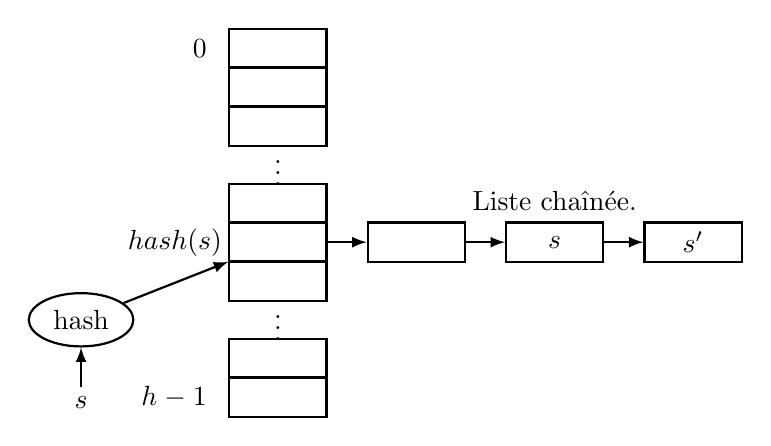
\begin{tikzpicture}[
          hashtable/.style={text width=1cm,minimum height=.5cm,node distance=14,align=center},
          hash/.style={draw,rectangle,hashtable},
          lab/.style={align=right,text width=1cm,node distance=40},
          list/.style={hash,node distance=50},
          every path/.style={draw,->,thick,>=latex}
        ]
        %hashtable
        \node[hash] (0) at (0,0) {};
        \node[below of = 0,hash] (1) {};
        \node[below of = 1,hash] (2) {};
        \node[below of = 2,hashtable] (3) {\vdots};
        \node[below of = 3,hash] (4) {};
        \node[below of = 4,hash] (5) {};
        \node[below of = 5,hash] (6) {};
        \node[below of = 6,hashtable] (7) {\vdots};
        \node[below of = 7,hash] (8) {};
        \node[below of = 8,hash] (9) {};

        %labels
        \node[left of = 0,lab] {$0$};
        \node[left of = 9,lab] {$h-1$};
        \node[left of = 5,lab] {$hash (s)$};

        %linked list
        \node[right of = 5,list] (51) {};
        \node[right of = 51,list] (52) {$s$};
        \node[right of = 52,list] (53) {$s'$};
        \path
        (5) edge (51)
        (51) edge (52)
        (52) edge (53)
        ;
        \node[above of = 52,node distance=15] {Liste chaînée.};

        %left part
        \node (s) at (-2.5,-4.5) {$s$};
        \node[above of = s,draw,ellipse,node distance=30] (hash) {hash};
        \path
        (s) edge (hash)
        (hash) edge (5)
        ;
    \end{tikzpicture}

      
    \subsubsection{Comment fonctionne la pile avec la table de hachage ?}
      Les blocs sont imbriqués les uns dans les autres. Lorsque des déclarations sont faîtes dans des blocs imbriqués il arrive que des symboles masquent des symboles déclararés dans des blocs parents.\\
      Quand dans un bloc un symbol est utilisé il fait référence à la première déclaration qui en a été faite. C'est à ce niveau que la pile est importante.\\

      Les niveaux de la pile représentent les niveaux d'imbrications. Dans cette pile, chacuns des niveaux ont une liste de symboles. C'est symboles sont représentés par leurs noms. Ainsi, grâce à la table de hachage il est aisé de récupérer l'instance correspondant au symbol en question.\\

      Lors de l'analyse, lorsqu'un bloc a été entièrement analysé, les déclarations de symboles qui y ont été réalisés deviennent obsolètes pour la suite de l'analyse. Il est nécessaire de faire du nettoyage dans la pile.\\

      Cette étape consiste à dépiler le bloc courant de la pile. Pour ce faire, le symbol en tête de liste pointée par ce bloc (celui le plus haut dans la pile) est supprimé. Cela doit être répété afin de vider la liste. La suppression est rapide puisque qu'il suffit de supprimer la tete de liste à chaque fois.\\
      Une fois la liste vide, le bloc peut être dépilé.

      \newpage

  \subsection{Exemple d'analyse sur un programme simple}
    \begin{multicols}{2}
        
        \begin{minted}[bgcolor=bg-gray]{c}
        { // bloc 1
          int a = 2;
          int b = a + 1; // b=3
         { // bloc 2
           int a = b + 2; // a=5
           { // bloc 3
             int b = a + 3; // b=8
             int c = a + b; // c=13
           }
           int c = a + b; // c=8
         }
         int c = a + b; // c=5
        }

        \end{minted}

      \columnbreak
        Ce programme réalise différents appels et et différentes déclarations au sein de plusieurs blocs imbriqués. Nous remarquons également que certaines variables sont masquées. Les commentaires nous aides à comprendre l'effet que cela implique sur le programme puisque l'expression a + b n'a pas la même valeur en fonction du bloc dans lequel elle est évaluée. Car ils contiennent des déclarations de a et de b qui masquent les précédentes.\\

        Déroulons pas à pas l'analyse des symboles.
       
    \end{multicols}
    % step 1
    \subsubsection{Première étape}
    \begin{multicols}{2}
        
        \begin{minted}[bgcolor=bg-gray]{c}
        { // bloc 1 <-----
          int a = 2; // @ref1
          int b = a + 1; // @ref2
         { // bloc 2
           int a = b + 2; // @ref3
           { // bloc 3
             int b = a + 3; // @ref4
             int c = a + b; // @ref5
           }
           int c = a + b; // @ref6
         }
         int c = a + b; // @ref7
        }

        \end{minted}

      \columnbreak
        L'analyse commence par le bloc 1. La table de hachage est vide et la pile également.
      \end{multicols}

      \begin{multicols}{2}
        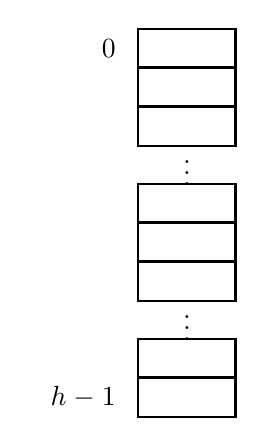
\begin{tikzpicture}[
            hashtable/.style={text width=1cm,minimum height=.5cm,node distance=14,align=center},
            hash/.style={draw,rectangle,hashtable},
            lab/.style={align=right,text width=1cm,node distance=40},
            list/.style={hash,node distance=50},
            every path/.style={draw,->,thick,>=latex}
          ]
          %hashtable
          \node[hash] (0) at (0,0) {};
          \node[below of = 0,hash] (1) {};
          \node[below of = 1,hash] (2) {};
          \node[below of = 2,hashtable] (3) {\vdots};
          \node[below of = 3,hash] (4) {};
          \node[below of = 4,hash] (5) {};
          \node[below of = 5,hash] (6) {};
          \node[below of = 6,hashtable] (7) {\vdots};
          \node[below of = 7,hash] (8) {};
          \node[below of = 8,hash] (9) {};

          %labels
          \node[left of = 0,lab] {$0$};
          \node[left of = 9,lab] {$h-1$};
      \end{tikzpicture}
      
      \columnbreak

      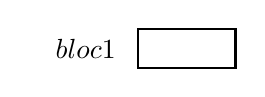
\begin{tikzpicture}[
            hashtable/.style={text width=1cm,minimum height=.5cm,node distance=14,align=center},
            hash/.style={draw,rectangle,hashtable},
            lab/.style={align=right,text width=1cm,node distance=40},
            list/.style={hash,node distance=50},
            every path/.style={draw,->,thick,>=latex}
          ]
          \node[hash] (0) at (0,0) {};
          
          %labels
          \node[left of = 0,lab] {$bloc 1$};
          
      \end{tikzpicture} 
    \end{multicols}

    % step 2
    \newpage
    \subsubsection{Deuxième étape}
    \begin{multicols}{2}
        
        \begin{minted}[bgcolor=bg-gray]{c}
        { // bloc 1
          int a = 2; // @ref1<-----
          int b = a + 1; // @ref2
         { // bloc 2
           int a = b + 2; // @ref3
           { // bloc 3
             int b = a + 3; // @ref4
             int c = a + b; // @ref5
           }
           int c = a + b; // @ref6
         }
         int c = a + b; // @ref7
        }

        \end{minted}

      \columnbreak
        Bloc 1:\\
        Déclaration de variable: int a = 2;\\
        %todo ajouter explications..
      \end{multicols}

      \begin{multicols}{2}
        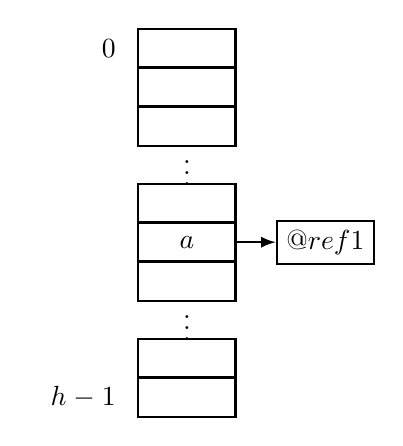
\begin{tikzpicture}[
            hashtable/.style={text width=1cm,minimum height=.5cm,node distance=14,align=center},
            hash/.style={draw,rectangle,hashtable},
            lab/.style={align=right,text width=1cm,node distance=40},
            list/.style={hash,node distance=50},
            every path/.style={draw,->,thick,>=latex}
          ]
          %hashtable
          \node[hash] (0) at (0,0) {};
          \node[below of = 0,hash] (1) {};
          \node[below of = 1,hash] (2) {};
          \node[below of = 2,hashtable] (3) {\vdots};
          \node[below of = 3,hash] (4) {};
          \node[below of = 4,hash] (5) {$a$};
          \node[below of = 5,hash] (6) {};
          \node[below of = 6,hashtable] (7) {\vdots};
          \node[below of = 7,hash] (8) {};
          \node[below of = 8,hash] (9) {};

          %labels
          \node[left of = 0,lab] {$0$};
          \node[left of = 9,lab] {$h-1$};

          %linked list
          \node[right of = 5,list] (51) {$@ref1$};
          \path
          (5) edge (51)
          ;

      \end{tikzpicture}
      
      \columnbreak
      
      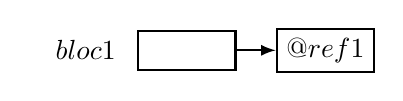
\begin{tikzpicture}[
            hashtable/.style={text width=1cm,minimum height=.5cm,node distance=14,align=center},
            hash/.style={draw,rectangle,hashtable},
            lab/.style={align=right,text width=1cm,node distance=40},
            list/.style={hash,node distance=50},
            every path/.style={draw,->,thick,>=latex}
          ]
          \node[hash] (0) at (0,0) {};
          
          %labels
          \node[left of = 0,lab] {$bloc 1$};

          %linked list
          \node[right of = 0,list] (01) {$@ref1$};
          \path
          (0) edge (01)
          ;
          
      \end{tikzpicture} 
    \end{multicols}

    % step 3
    \subsubsection{Troisième étape}
    \begin{multicols}{2}
        
        \begin{minted}[bgcolor=bg-gray]{c}
        { // bloc 1
          int a = 2; //@ref1
          int b = a + 1; // @ref2 <-----
         { // bloc 2
           int a = b + 2; // @ref3
           { // bloc 3
             int b = a + 3; // @ref4
             int c = a + b; // @ref5
           }
           int c = a + b; // @ref6
         }
         int c = a + b; // @ref7
        }

        \end{minted}

      \columnbreak
        Bloc 1:\\
        Déclaration de variable: int b = a + 1;\\
        % todo : ajouter explications...
      \end{multicols}

      \begin{multicols}{2}
        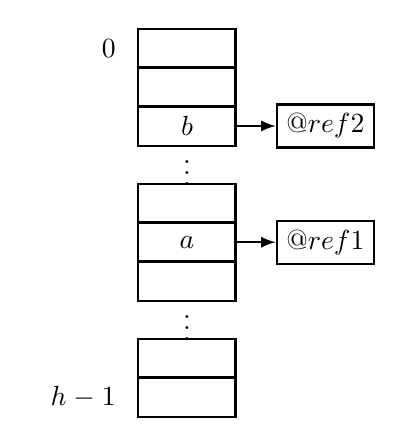
\begin{tikzpicture}[
            hashtable/.style={text width=1cm,minimum height=.5cm,node distance=14,align=center},
            hash/.style={draw,rectangle,hashtable},
            lab/.style={align=right,text width=1cm,node distance=40},
            list/.style={hash,node distance=50},
            every path/.style={draw,->,thick,>=latex}
          ]
          %hashtable
          \node[hash] (0) at (0,0) {};
          \node[below of = 0,hash] (1) {};
          \node[below of = 1,hash] (2) {$b$};
          \node[below of = 2,hashtable] (3) {\vdots};
          \node[below of = 3,hash] (4) {};
          \node[below of = 4,hash] (5) {$a$};
          \node[below of = 5,hash] (6) {};
          \node[below of = 6,hashtable] (7) {\vdots};
          \node[below of = 7,hash] (8) {};
          \node[below of = 8,hash] (9) {};

          %labels
          \node[left of = 0,lab] {$0$};
          \node[left of = 9,lab] {$h-1$};

          %linked list
          \node[right of = 5,list] (51) {$@ref1$};
          \node[right of = 2,list] (21) {$@ref2$};
          \path
          (5) edge (51)
          (2) edge (21)
          ;

      \end{tikzpicture}
      
      \columnbreak
      
      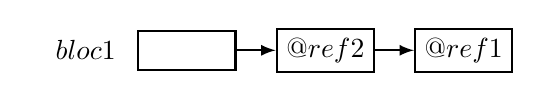
\begin{tikzpicture}[
            hashtable/.style={text width=1cm,minimum height=.5cm,node distance=14,align=center},
            hash/.style={draw,rectangle,hashtable},
            lab/.style={align=right,text width=1cm,node distance=40},
            list/.style={hash,node distance=50},
            every path/.style={draw,->,thick,>=latex}
          ]
          \node[hash] (0) at (0,0) {};
          
          %labels
          \node[left of = 0,lab] {$bloc 1$};

          %linked list
          \node[right of = 0,list] (01) {$@ref2$};
          \node[right of = 01,list] (02) {$@ref1$};
          \path
          (0) edge (01)
          (01) edge (02)
          ;
          
      \end{tikzpicture} 
    \end{multicols}

    % step 4
    \subsubsection{Quatrième étape}
    \begin{multicols}{2}
        
        \begin{minted}[bgcolor=bg-gray]{c}
        { // bloc 1
          int a = 2; // @ref1
          int b = a + 1; // @ref2
         { // bloc 2 <-----
           int a = b + 2; // @ref3
           { // bloc 3
             int b = a + 3; // @ref4
             int c = a + b; // @ref5
           }
           int c = a + b; // @ref6
         }
         int c = a + b; // @ref7
        }

        \end{minted}

      \columnbreak
        Bloc 2: Création d'une liste vide sur la pile
        
      \end{multicols}

      \begin{multicols}{2}
        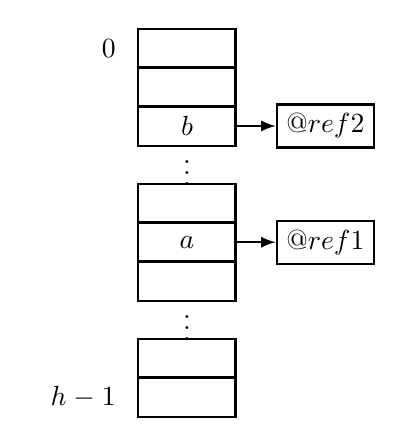
\begin{tikzpicture}[
            hashtable/.style={text width=1cm,minimum height=.5cm,node distance=14,align=center},
            hash/.style={draw,rectangle,hashtable},
            lab/.style={align=right,text width=1cm,node distance=40},
            list/.style={hash,node distance=50},
            every path/.style={draw,->,thick,>=latex}
          ]
          %hashtable
          \node[hash] (0) at (0,0) {};
          \node[below of = 0,hash] (1) {};
          \node[below of = 1,hash] (2) {$b$};
          \node[below of = 2,hashtable] (3) {\vdots};
          \node[below of = 3,hash] (4) {};
          \node[below of = 4,hash] (5) {$a$};
          \node[below of = 5,hash] (6) {};
          \node[below of = 6,hashtable] (7) {\vdots};
          \node[below of = 7,hash] (8) {};
          \node[below of = 8,hash] (9) {};

          %labels
          \node[left of = 0,lab] {$0$};
          \node[left of = 9,lab] {$h-1$};

          %linked list
          \node[right of = 5,list] (51) {$@ref1$};
          \node[right of = 2,list] (21) {$@ref2$};
          \path
          (5) edge (51)
          (2) edge (21)
          ;

      \end{tikzpicture}
      
      \columnbreak
      
      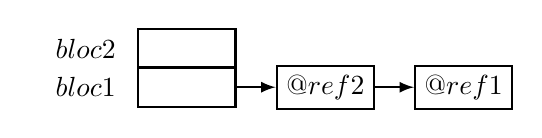
\begin{tikzpicture}[
            hashtable/.style={text width=1cm,minimum height=.5cm,node distance=14,align=center},
            hash/.style={draw,rectangle,hashtable},
            lab/.style={align=right,text width=1cm,node distance=40},
            list/.style={hash,node distance=50},
            every path/.style={draw,->,thick,>=latex}
          ]
          \node[hash] (1) at (0,0) {};
          \node[below of = 1,hash] (0) {};
          
          %labels
          \node[left of = 0,lab] {$bloc 1$};
          \node[left of = 1,lab] {$bloc 2$};

          %linked list
          \node[right of = 0,list] (01) {$@ref2$};
          \node[right of = 01,list] (02) {$@ref1$};
          \path
          (0) edge (01)
          (01) edge (02)
          ;
          
      \end{tikzpicture} 
    \end{multicols}

    % step 5
    \subsubsection{Cinquième étape}
    \begin{multicols}{2}
        
        \begin{minted}[bgcolor=bg-gray]{c}
        { // bloc 1
          int a = 2; // @ref1
          int b = a + 1; // @ref2
         { // bloc 2 
           int a = b + 2; // @ref3 <-----
           { // bloc 3
             int b = a + 3; // @ref4
             int c = a + b; // @ref5
           }
           int c = a + b; // @ref6
         }
         int c = a + b; // @ref7
        }

        \end{minted}

      \columnbreak
        Déclaration de a qui masque celle précendente.
        %todo ajouter explications
        
      \end{multicols}

      \begin{multicols}{2}
        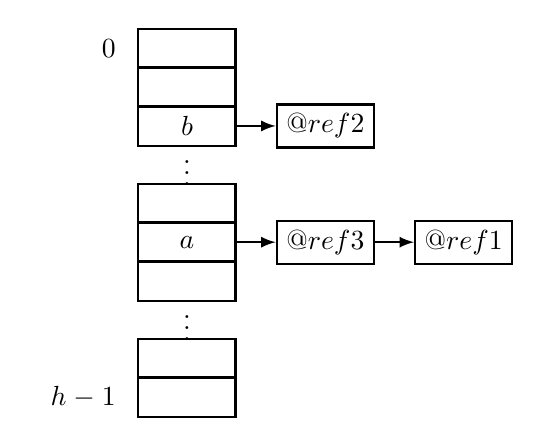
\begin{tikzpicture}[
            hashtable/.style={text width=1cm,minimum height=.5cm,node distance=14,align=center},
            hash/.style={draw,rectangle,hashtable},
            lab/.style={align=right,text width=1cm,node distance=40},
            list/.style={hash,node distance=50},
            every path/.style={draw,->,thick,>=latex}
          ]
          %hashtable
          \node[hash] (0) at (0,0) {};
          \node[below of = 0,hash] (1) {};
          \node[below of = 1,hash] (2) {$b$};
          \node[below of = 2,hashtable] (3) {\vdots};
          \node[below of = 3,hash] (4) {};
          \node[below of = 4,hash] (5) {$a$};
          \node[below of = 5,hash] (6) {};
          \node[below of = 6,hashtable] (7) {\vdots};
          \node[below of = 7,hash] (8) {};
          \node[below of = 8,hash] (9) {};

          %labels
          \node[left of = 0,lab] {$0$};
          \node[left of = 9,lab] {$h-1$};

          %linked list
          \node[right of = 5,list] (51) {$@ref3$};
          \node[right of = 51,list] (52) {$@ref1$};
          \node[right of = 2,list] (21) {$@ref2$};
          \path
          (5) edge (51)
          (2) edge (21)
          (51) edge (52)
          ;

      \end{tikzpicture}
      
      \columnbreak
      
      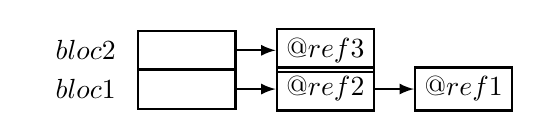
\begin{tikzpicture}[
            hashtable/.style={text width=1cm,minimum height=.5cm,node distance=14,align=center},
            hash/.style={draw,rectangle,hashtable},
            lab/.style={align=right,text width=1cm,node distance=40},
            list/.style={hash,node distance=50},
            every path/.style={draw,->,thick,>=latex}
          ]
          \node[hash] (1) at (0,0) {};
          \node[below of = 1,hash] (0) {};
          
          %labels
          \node[left of = 0,lab] {$bloc 1$};
          \node[left of = 1,lab] {$bloc 2$};

          %linked list
          \node[right of = 0,list] (01) {$@ref2$};
          \node[right of = 01,list] (02) {$@ref1$};

          \node[right of = 1,list] (10) {$@ref3$};
          \path
          (0) edge (01)
          (01) edge (02)
          (1) edge (10)
          ;
          
      \end{tikzpicture} 
    \end{multicols}

    % step 6
    \subsubsection{Sixième étape}
    \begin{multicols}{2}
        
        \begin{minted}[bgcolor=bg-gray]{c}
        { // bloc 1
          int a = 2; // @ref1
          int b = a + 1; // @ref2
         { // bloc 2 
           int a = b + 2; // @ref3
           { // bloc 3 <-----
             int b = a + 3; // @ref4
             int c = a + b; // @ref5
           }
           int c = a + b; // @ref6
         }
         int c = a + b; // @ref7
        }

        \end{minted}

      \columnbreak
        Création d'une liste vide sur la pile pour le bloc3
        %todo ajouter explications
        
      \end{multicols}

      \begin{multicols}{2}
        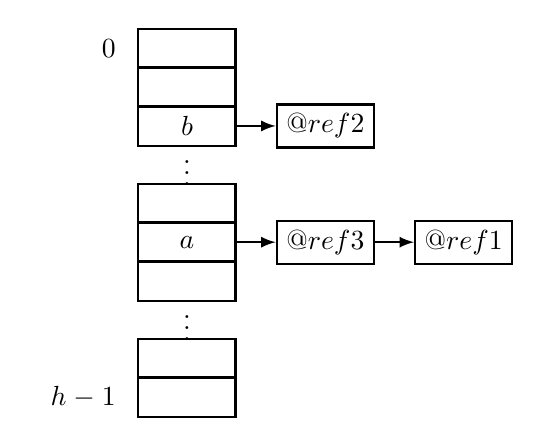
\begin{tikzpicture}[
            hashtable/.style={text width=1cm,minimum height=.5cm,node distance=14,align=center},
            hash/.style={draw,rectangle,hashtable},
            lab/.style={align=right,text width=1cm,node distance=40},
            list/.style={hash,node distance=50},
            every path/.style={draw,->,thick,>=latex}
          ]
          %hashtable
          \node[hash] (0) at (0,0) {};
          \node[below of = 0,hash] (1) {};
          \node[below of = 1,hash] (2) {$b$};
          \node[below of = 2,hashtable] (3) {\vdots};
          \node[below of = 3,hash] (4) {};
          \node[below of = 4,hash] (5) {$a$};
          \node[below of = 5,hash] (6) {};
          \node[below of = 6,hashtable] (7) {\vdots};
          \node[below of = 7,hash] (8) {};
          \node[below of = 8,hash] (9) {};

          %labels
          \node[left of = 0,lab] {$0$};
          \node[left of = 9,lab] {$h-1$};

          %linked list
          \node[right of = 5,list] (51) {$@ref3$};
          \node[right of = 51,list] (52) {$@ref1$};
          \node[right of = 2,list] (21) {$@ref2$};
          \path
          (5) edge (51)
          (2) edge (21)
          (51) edge (52)
          ;

      \end{tikzpicture}
      
      \columnbreak
      
      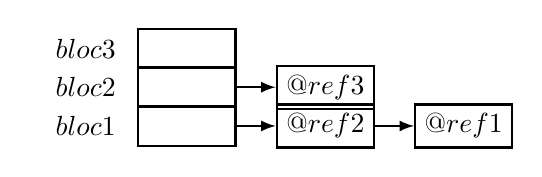
\begin{tikzpicture}[
            hashtable/.style={text width=1cm,minimum height=.5cm,node distance=14,align=center},
            hash/.style={draw,rectangle,hashtable},
            lab/.style={align=right,text width=1cm,node distance=40},
            list/.style={hash,node distance=50},
            every path/.style={draw,->,thick,>=latex}
          ]
          \node[hash] (2) at (0,0) {};
          \node[below of = 2,hash] (1) {};
          \node[below of = 1,hash] (0) {};
          
          %labels
          \node[left of = 0,lab] {$bloc 1$};
          \node[left of = 1,lab] {$bloc 2$};
          \node[left of = 2,lab] {$bloc 3$};

          %linked list
          \node[right of = 0,list] (01) {$@ref2$};
          \node[right of = 01,list] (02) {$@ref1$};

          \node[right of = 1,list] (10) {$@ref3$};
          \path
          (0) edge (01)
          (01) edge (02)
          (1) edge (10)
          ;
          
      \end{tikzpicture} 
    \end{multicols}

    % step 7
    \subsubsection{Septième étape}
    \begin{multicols}{2}
        
        \begin{minted}[bgcolor=bg-gray]{c}
        { // bloc 1
          int a = 2; // @ref1
          int b = a + 1; // @ref2
         { // bloc 2 
           int a = b + 2; // @ref3
           { // bloc 3
             int b = a + 3; // @ref4 <-----
             int c = a + b; // @ref5 <-----
           }
           int c = a + b; // @ref6
         }
         int c = a + b; // @ref7
        }

        \end{minted}

      \columnbreak
        Puisque le fonctionnement est similaire aux étapes précendentes, nous avons condensé les deux étapes une seule sur le schéma.\\

        Déclaration masquante de b et déclaration locale de c.
        %todo ajouter explications
        
      \end{multicols}

      \begin{multicols}{2}
        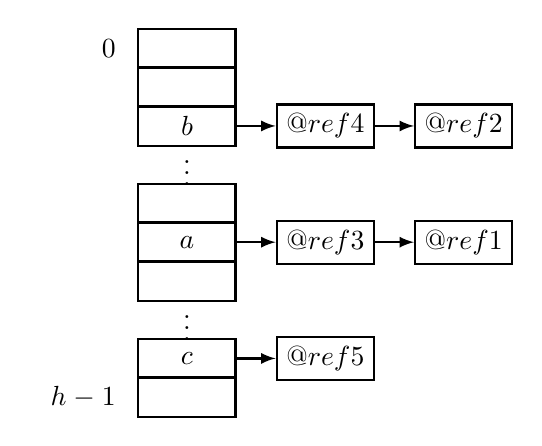
\begin{tikzpicture}[
            hashtable/.style={text width=1cm,minimum height=.5cm,node distance=14,align=center},
            hash/.style={draw,rectangle,hashtable},
            lab/.style={align=right,text width=1cm,node distance=40},
            list/.style={hash,node distance=50},
            every path/.style={draw,->,thick,>=latex}
          ]
          %hashtable
          \node[hash] (0) at (0,0) {};
          \node[below of = 0,hash] (1) {};
          \node[below of = 1,hash] (2) {$b$};
          \node[below of = 2,hashtable] (3) {\vdots};
          \node[below of = 3,hash] (4) {};
          \node[below of = 4,hash] (5) {$a$};
          \node[below of = 5,hash] (6) {};
          \node[below of = 6,hashtable] (7) {\vdots};
          \node[below of = 7,hash] (8) {$c$};
          \node[below of = 8,hash] (9) {};

          %labels
          \node[left of = 0,lab] {$0$};
          \node[left of = 9,lab] {$h-1$};

          %linked list
          \node[right of = 5,list] (51) {$@ref3$};
          \node[right of = 51,list] (52) {$@ref1$};
          \node[right of = 2,list] (21) {$@ref4$};
          \node[right of = 21,list] (22) {$@ref2$};

          \node[right of = 8,list] (81) {$@ref5$};
          \path
          (5) edge (51)
          (2) edge (21)
          (21) edge (22)
          (8) edge (81)
          (51) edge (52)
          ;

      \end{tikzpicture}
      
      \columnbreak
      
      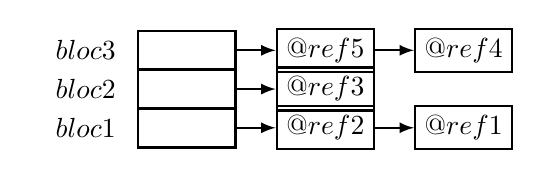
\begin{tikzpicture}[
            hashtable/.style={text width=1cm,minimum height=.5cm,node distance=14,align=center},
            hash/.style={draw,rectangle,hashtable},
            lab/.style={align=right,text width=1cm,node distance=40},
            list/.style={hash,node distance=50},
            every path/.style={draw,->,thick,>=latex}
          ]
          \node[hash] (2) at (0,0) {};
          \node[below of = 2,hash] (1) {};
          \node[below of = 1,hash] (0) {};
          
          %labels
          \node[left of = 0,lab] {$bloc 1$};
          \node[left of = 1,lab] {$bloc 2$};
          \node[left of = 2,lab] {$bloc 3$};

          %linked list
          \node[right of = 0,list] (01) {$@ref2$};
          \node[right of = 01,list] (02) {$@ref1$};

          \node[right of = 1,list] (10) {$@ref3$};
          
          \node[right of = 2,list] (20) {$@ref5$};
          \node[right of = 20,list] (21) {$@ref4$};
          \path
          (0) edge (01)
          (01) edge (02)
          (1) edge (10)

          (2) edge (20)
          (20) edge (21)
          ;
          
      \end{tikzpicture} 
    \end{multicols}

    % step 8
    \subsubsection{Huitième étape}
    \begin{multicols}{2}
        
        \begin{minted}[bgcolor=bg-gray]{c}
        { // bloc 1
          int a = 2; // @ref1
          int b = a + 1; // @ref2
         { // bloc 2 
           int a = b + 2; // @ref3
           { // bloc 3
             int b = a + 3; // @ref4
             int c = a + b; // @ref5
           } <-----
           int c = a + b; // @ref6
         }
         int c = a + b; // @ref7
        }

        \end{minted}

      \columnbreak
        Ici on sort du bloc3 donc on va dépiler le bloc3 de la pile.\\
        On récupère la tete de liste du bloc courant (bloc 3) qui est la référence vers un élément de la table de hachage. Ensuite on supprime cet élément de la table de hachage. On supprime également cet élément de la liste du bloc courant.\\
        Quand la liste est vide alors on dépile le bloc3 de la pile.
        
        
      \end{multicols}

      \begin{multicols}{2}
        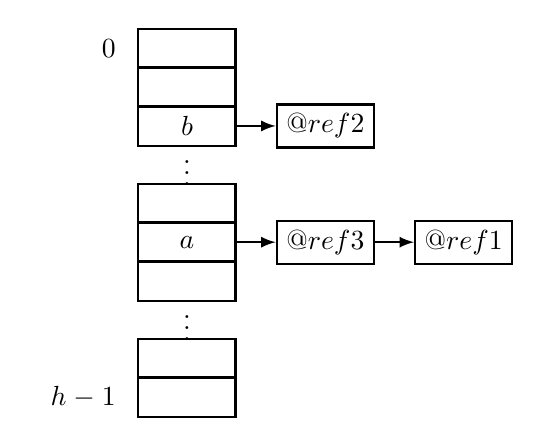
\begin{tikzpicture}[
            hashtable/.style={text width=1cm,minimum height=.5cm,node distance=14,align=center},
            hash/.style={draw,rectangle,hashtable},
            lab/.style={align=right,text width=1cm,node distance=40},
            list/.style={hash,node distance=50},
            every path/.style={draw,->,thick,>=latex}
          ]
          %hashtable
          \node[hash] (0) at (0,0) {};
          \node[below of = 0,hash] (1) {};
          \node[below of = 1,hash] (2) {$b$};
          \node[below of = 2,hashtable] (3) {\vdots};
          \node[below of = 3,hash] (4) {};
          \node[below of = 4,hash] (5) {$a$};
          \node[below of = 5,hash] (6) {};
          \node[below of = 6,hashtable] (7) {\vdots};
          \node[below of = 7,hash] (8) {};
          \node[below of = 8,hash] (9) {};

          %labels
          \node[left of = 0,lab] {$0$};
          \node[left of = 9,lab] {$h-1$};

          %linked list
          \node[right of = 5,list] (51) {$@ref3$};
          \node[right of = 51,list] (52) {$@ref1$};
          \node[right of = 2,list] (21) {$@ref2$};
          
          \path
          (5) edge (51)
          (2) edge (21)
          
          (51) edge (52)
          ;

      \end{tikzpicture}
      
      \columnbreak
      
      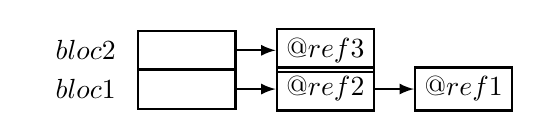
\begin{tikzpicture}[
            hashtable/.style={text width=1cm,minimum height=.5cm,node distance=14,align=center},
            hash/.style={draw,rectangle,hashtable},
            lab/.style={align=right,text width=1cm,node distance=40},
            list/.style={hash,node distance=50},
            every path/.style={draw,->,thick,>=latex}
          ]
          \node[hash] (1) at (0,0) {};
          \node[below of = 1,hash] (0) {};
          
          %labels
          \node[left of = 0,lab] {$bloc 1$};
          \node[left of = 1,lab] {$bloc 2$};
          

          %linked list
          \node[right of = 0,list] (01) {$@ref2$};
          \node[right of = 01,list] (02) {$@ref1$};

          \node[right of = 1,list] (10) {$@ref3$};
          
          
          \path
          (0) edge (01)
          (01) edge (02)
          (1) edge (10)
          ;
          
      \end{tikzpicture} 
    \end{multicols}


\section{Étapes de l'analyse sémantique}
 \subsection{Liste des vérifications à réaliser}
  Au cours de l’analyse sémantique il faudra effectuer de nombreuses vérifications. Voici la liste des
  éléments à vérifier pour compléter une partie de l’analyse sémantique (en effet il y a également une
  partie décoration) ; dans le désordre : % a remettre dans l'ordre..
  \begin{itemize}
    \item Déclaration de variable avec un type existant
    \item Affectation avec un typage correct
    \item Comparaison entre type correct (cast implicite autorisé)
    \item Pas de cycles dans l’héritage
    \item Appelle de méthode « static » au sein d’une méthode => la méthode doit être « static »
    \item Présence de méthode « abstract » dans une classe => la classe doit être « abstract »
    \item Définition de toutes les méthodes lors de l’implémentation d’une interface
    \item Appelle de méthode correcte (méthode existante + paramètres valide)
    \item Return présent et correctement typé dans les méthodes avec un type de retour != void
    \item Appelle de variable correcte (variable déclarée et visible au moment de l’appel)
    \item Pas de modification sur une variable « final »
    \item Pas de nommage identique pour les classes
  \end{itemize}

 \subsection{Les différentes phases de l’analyse sémantiques}
  Pour réaliser une analyse sémantique complète plusieurs passes dans l’arbre sont nécessaires.
  Nous allons avoir besoins de parcourir l’arbre 3 (ou 4fois)

  \subsubsection{Phase 1}
  \begin{itemize}
    \item Enregistrer chaque classe comme un type
  \end{itemize}
  \subsubsection{Phase 2}
  \begin{itemize}
    \item Décorer chaque classe avec le type de sa classe mère et de ses interfaces
    \item Décorer les attributs
    \item Décorer les méthodes :
      \begin{itemize}
        \item Associer une référence aux paramètres ( et type de retour ?)
        \item Calcul et enregistrement de la signature complète
      \end{itemize}
    
  \end{itemize}
  \subsubsection{Phase 2 (suite) ou 3}
  \begin{itemize}
    \item Création des interfaces publiques pour chaque classe (listes des méthodes et attributs
  complètes).
  \end{itemize}
  \subsubsection{Phase 3 ou 4 (selon choix précédent)}
  \begin{itemize}
    \item Analyse sémantique des corps de méthodes
  \end{itemize}

 \section{Interface de la table des symboles}
    \begin{minted}[bgcolor=bg-gray]{cpp}
    /**
     * Interface ITableOfSymbol.
     * Specifie les operations sur la table des symboles.
     */
    class ITableOfSymbol{public:
      // Requete

      /**
       * Retourne l'instance representant le symbol en fonction de son nom.
       * @param sym Nom du symbol.
       */
      virtual SemanticPtr* getSymbol(String sym) = 0;

      // Commandes

      /**
       * Place le curseur interne sur un nouveau bloc.
       * Toutes les futures operations se feront sur ce bloc.
       */
      virtual void enterBloc() = 0;

      /**
       * Deplace le curseur interne sur le bloc precedent.
       * Toutes les futures operations se feront sur ce bloc.
       */
      virtual void exitBloc() = 0;

      /**
       * Ajoute une definition de symbol dans la table des symboles.
       * @param sym Nom du symbol
       * @param sptr pointeur sur l'instance qui represente le symbol.
       */
      virtual void addSymbol(String sym, SemanticPtr* sptr) = 0;
    }
    \end{minted}

  \subsection{enterBloc}
    La fonction enterBloc doit être appellée lorsque l'analyseur sémantique entre dans un bloc. Ainsi un nouveau bloc sera empilé sur la pile. Les recherches de symboles se feront en prenant en compte les niveaux d'imbrications des blocs.
  \subsection{exitBloc}
   Réciproquement, lorsque l'analyseur sémantique quitte un bloc, la fonction exitBloc doit être appellée. Cela permet de dépiler un bloc de la pile afin de supprimer les déclarations qui sont obsolètes car innaccessibles depuis l'exterieur du bloc.
\end{document}
